\lab{Introduction to NumPy}{Introduction to NumPy} 
\label{lab:NumPy}
\objective{Python's NumPy and SciPy packages make Python an ideal language for scientific computing. NumPy is a package for manipulating data with multi-dimensional vectors, and SciPy is a higher-level library built on NumPy. Both packages will be used extensively in almost every lab hereafter in this curriculum. In this lab we introduce basic NumPy data structures and operations as a first step to numerical computing in Python.}

%\footnote{SciPy is also the name of a Python coding environment that includes the NumPy and SciPy libraries, as well as IPython, matplotlib, and other tools.}

% Lab Outline
% - Arrays
%     - [x] What is an array?
%     - [x] How to initialize a simple custom array
%     - [x] **Problem 1**: Matrix Equation 1
%     - [x] Basic array operations +, -, *, / component-wise
%     - [x] **Problem 2**: Matrix Equation 2 (Cayley-Hamilton preview)
%     - Data Types
%         - [x] How to initialize an array with a certain type
%         - [x] Changing the type of an array's elements
%         - [x] Warning: precision limits on data types (int16)
%     - Special Creation routines
%         - [x] `zeros()`, `ones()`, `eye()`, `identity()`, `full()`, etc.
%         - [x] `diag()`, `tril()`, `triu()`
%         - [x] **Problem 3**: Matrix Equation 3
% - Data Access
%     - [x] Slicing Revisited (refer to the visual guide included at the end of the lab)
%     - [x] Warning: views vs copies (mutability, `np.copy()`)
%     - [x] Fancy Indexing and Masks
%     - [x] **Problem 4**: Use fancy indexing to make all entries of a matrix nonnegative (something harder!!)
% - Array Manipulation
%     - [x] `reshape()`, `ravel()` / `flatten()`, `transpose()`
%     - [x] `hstack()`, `vstack()`, `column_stack()`
%     - [x] Note / Warning: All 1D numpy arrays are flat! (`np.newaxis`)
%     - [x] **Problem 5**: A final, hardest matrix equation (block matrices)
%     - [ ] Array Broadcasting
% - Universal Functions / Avoid Looping!!
%     - NumPy uses C and Fortran to be SPEEDY!
%     - [ ] `max()`, `min()`, `argmax()`, `argmin()`
%     - [ ] The `axis` argument.
%     - [ ] **Problem 6**: Laplace's equation (needs rewording and algorithm box, but it's legit)
% - Additional Material
%     - Random Sampling
%     - Saving / Loading arrays
%     - Iterating through arrays
% - Visual Reference Guide
%     - [x] Data Access
%     - [x] Slicing
%     - [x] Stacking
%     - [ ] Broadcasting

\section*{Arrays} % ===========================================================

In many algorithms, data can be represented mathematically as a \emph{vector} or a \emph{matrix}.
Conceptually, a vector is just a list of numbers and a matrix is a two-dimensional list of numbers.
Therefore, we might try to represent a vector as a Python list and a matrix as a list of lists.
However, even basic linear algebra operations like matrix multiplication are cumbersome to implement and slow to execute when we store data this way.
The \emph{NumPy} module\footnote{NumPy is \emph{not} part of the standard library, but it is included in most Python distributions.} offers a much better solution.

The basic object in NumPy is the \emph{array}, which is conceptually similar to a matrix.
The NumPy array class is called \li{ndarray} (for ``$n$-dimensional array'').
The simplest way to explicitly create a 1-D \li{ndarray} is to define a list, then cast that list as an \li{ndarray} with NumPy's \li{array()} function.

\begin{lstlisting}
>>> import numpy as np
# Create a 1-D array by passing a list into NumPy's array() function.
>>> np.array([8, 4, 6, 0, 4])
array([8, 4, 6, 0, 4])
\end{lstlisting}
The alias \li{np} is standard in the Python community.

An \li{ndarray} can have arbitrarily many dimensions.
A 2-D array is a 1-D array of 1-D arrays, and more generally, an $n$-dimensional array is a 1-D array of $(n-1)$-dimensional arrays.
Each dimension is called an \emph{axis}.
For a 2-D array, the 0-axis indexes the rows and the 1-axis indexes the columns.
Elements are accessed using brackets and indices (like a regular list), and the axes are separated by commas.

\begin{lstlisting}
# Create a 2-D array by passing a list of lists into array().
>>> A = np.array([[1, 2, 3], [4, 5, 6]])
>>> print(A)
[[1, 2, 3],
 [4, 5, 6]]

# Access elements of the array with brackets.
>>> print A[0, 1], A[1, 2]
2 6

# The elements of a 2-D array are 1-D arrays.
>>> A[0]
array([1, 2, 3])
\end{lstlisting}

\begin{problem} % Problem 1: Matrix Multiplication
NumPy's \li{dot()} function performs matrix multiplication. % In Python 3.5, we can use the @ operator to perform matrix multiplication.
Write a function that defines the following matrices as NumPy arrays.
\begin{align*}
A = \left(\begin{array}{rrr}
3 & -1 &  4 \\ 
1 &  5 & -9 \end{array}\right)
&&
B = \left(\begin{array}{cccc}
2 &  6 & -5 &  3\\
5 & -8 &  9 &  7\\
9 & -3 & -2 & -3\end{array}\right)
\end{align*}
Return the matrix product $AB$.
% Solution:
% array([[ 37,  14, -32, -10],
%        [-54,  -7,  58,  65]])

NumPy has excellent documentation.
For examples of array initialization and matrix multiplication, use IPython's object introspection feature to look up the documentation for \li{np.ndarray}, \li{np.array()} and \li{np.dot()}.
\begin{lstlisting}
In [1]: import numpy as np
In [2]: np.array?       # press 'Enter'
\end{lstlisting}
\label{prob:simple1}
\end{problem}

\subsection*{Array Attributes} % ----------------------------------------------
An \li{ndarray} object has several attributes, some of which are listed below.

\begin{table}[H] % Important ndarray Attributes
\centering 
\begin{tabular}{c|l}%{10cm}}
    Attribute & Description \\
    \hline \li{dtype} & The type of the elements in the array. \\
    \li{ndim} & The number of axes (dimensions) of the array. \\
    \li{shape} & A tuple of integers indicating the size in each dimension. \\
    \li{size} & The total number of elements in the array. \\
\end{tabular}
% \caption{A few of the attributes of NumPy arrays.}
\label{table:ndarrayattrs}
\end{table}
\begin{lstlisting}
>>> A = np.array([[1, 2, 3], [4, 5, 6]])
>>> A.ndim
2
>>> A.shape
(2, 3)
>>> A.size
6
\end{lstlisting}

Note that the \li{ndim} is the number of entries in \li{shape}, and the
the \li{size} of the array is the product of the entries of \li{shape}.

\subsection*{Basic Array Operations} % ----------------------------------------

NumPy arrays behave differently with respect to the binary arithmetic operators \li{+} and \li{*} than Python lists do.
For lists, \li{+} concatenates two lists and \li{*} replicates a list by a scalar amount (strings also behave this way).

\begin{lstlisting}
# Addition performs list concatenation.
>>> [1, 2, 3] + [4, 5, 6]
[1, 2, 3, 4, 5, 6]

# Mutliplication concatenates a list with itself a given number of times.
>>> [1, 2, 3] * 4
[1, 2, 3, 1, 2, 3, 1, 2, 3, 1, 2, 3]
\end{lstlisting}

These operations are element-wise for NumPy arrays, so that arrays behave the same way that vectors and matrices behave mathematically.

\begin{lstlisting}
>>> x = np.array([1, 2, 3])
>>> y = np.array([4, 5, 6])

# Addition or multiplication by a scalar acts on each element of the array.
>>> x + 2
array([3, 4, 5])
>>> x * 4
array([ 4,  8, 12])

# Add two arrays together (component-wise).
>>> x + y
array([5, 7, 9])

# Multiply two arrays together (component-wise).
>>> x * y
array([ 4, 10, 18])
\end{lstlisting}

% Subtraction and division also perform element-wise operations for arrays.
Apart from being syntactically convenient, element-wise NumPy operations also execute significantly faster than element-wise list operations.

\begin{comment} % Old demonstration, overkill.
\begin{lstlisting}
In [1]: import numpy as np
In [2]: from random import random

# Make two lists of 10000 random entries and corresponding NumPy arrays.
In [3]: a = [random() for i in xrange(10000)]
In [4]: b = [random() for i in xrange(10000)]
In [5]: A, B = np.array(a), np.array(b)

In [6]: %timeit [x + y for x,y in zip(a,b)]
100 loops, best of 3: 2.02 milisecons per loop          # .00202 seconds.

In [7]: %timeit A + B
100000 loops, best of 3: 92.9 microseconds per loop     # .0000929 seconds.
\end{lstlisting}

\begin{lstlisting}
# For lists, + performs concatenation (not addition) and * is not defined.
>>> a = [1, 2, 3]
>>> b = [4, 5, 6]
>>> a + b
[1, 2, 3, 4, 5, 6]
>>> a * b
<<TypeError: cannot multiply sequence by non-int of type 'list'>>

# Element-wise operations for lists are possible, but cumbersome.
>>> [x + y for x, y in zip(a, b)]
[5, 7, 9]
>>> [x * y for x, y in zip(a, b)]
[4, 10, 18]

# With NumPy arrays, addition and multiplication are element-wise.
>>> a = np.array(a)             # Cast 'a' and 'b' as NumPy arrays.
>>> b = np.array(b)
>>> a + b
array([5, 7, 9])
>>> a * b
array([4, 10, 18])
\end{lstlisting}

Apart from being syntactically convenient, element-wise NumPy operations are also significantly faster than element-wise list operations.

\begin{lstlisting}
>>> from time import time
>>> from random import random

# Make two random lists with 10000 entries each.
>>> a = [random() for i in xrange(10000)]
>>> b = [random() for i in xrange(10000)]

# Time the element-wise addition for lists.
>>> start = time()
>>> [x + y for x, y in zip(a, b))]
>>> list_time = time() - start

# Cast each list as a NumPy array.
>>> A, B = np.array(a), np.array(b)

# Time the element-wise addition for arrays.
>>> start = time()
>>> a + b
>>> array_time = time() - start

# Report the times.
>>> print list_time, array_time
0.0030951499939 0.000310897827148
\end{lstlisting}
\end{comment}

\begin{problem} % Simple Matrix Equation 2 (Cayley Hamilton)
Write a function that defines the following matrix as a NumPy array.
\[
A = \left(\begin{array}{rrr}
3 & 1 & 4\\ 
1 & 5 & 9 \\
-5 & 3 & 1 \end{array}\right)
\]
Return the matrix $-A^3 + 9A^2 - 15A$.
In this context, $A^2 = AA$ (the matrix product).

The somewhat surprising result is a demonstration of the Cayley-Hamilton theorem, which will be discussed late in the curriculum.
\label{prob:simple2}
\end{problem}

\subsection*{Data Types} % ----------------------------------------------------

Unlike native Python data structures, \textbf{all elements of a NumPy array must have the same data type}. 
The data types used by NumPy arrays are machine-native and avoid the overhead of Python objects, meaning that they are faster to compute with.
Thus NumPy's \li{np.float64} and Python's standard \li{float} are not the same; the former has been optimized to speed up numerical computations.
NumPy's more common numerical data types are listed below in Table \ref{table:numpytypes}.

\begin{table}[H] % Numpy Data Types
\centering
\begin{tabular}{l|l}
Data type & Description 
\\ \hline 
\li{bool_} & Boolean \\ 
\li{int8} & 8-bit integer \\
\li{int16} & 16-bit integer \\
\li{int32} & 32-bit integer \\
\li{int64} & 64-bit integer \\ 
\li{uint8} & Unsigned 8-bit integer \\ 
\li{uint16} & Unsigned 16-bit integer \\ 
\li{uint32} & Unsigned 32-bit integer \\
\li{uint64} & Unsigned 64-bit integer \\ 
\li{float16} & Half-precision float \\ 
\li{float32} & Single-precision float \\ 
\li{float64} & Double-precision float (default type for most computations)\\ 
\li{complex64} & Complex number represented by two single-precision floats \\ 
\li{complex128} & Complex number represented by two double-precision floats
\end{tabular}
\caption{Native numerical data types available in NumPy. The numbers on these types, such as the 16 on \li{int16}, indicates the number of bits used by the machine to store the number. Thus \li{float64} is more precise, but more computationally expensive, than \li{float16}.}
\label{table:numpytypes} 
\end{table}

We specify the data type of an array as it is created with the keyword argument \li{dtype}.
If unspecified, then the type will be determined as the minimum type required to hold the objects in the provided sequence.
To change an existing array's type, use the array's \li{astype()} method.

\begin{lstlisting}
# A list of integers becomes an array of integers.
>>> x = np.array([0, 1, 2, 3, 4])
>>> print(x)
[0 1 2 3 4]
>>> x.dtype
<<dtype('int64')>>

# Change the data type to one of NumPy's float types.
>>> x = x.astype(np.float64)
>>> print(x)
[ 0.  1.  2.  3.  4.]
>>> x.dtype
<<dtype('float64')>>
\end{lstlisting}

\begin{warn}
The default data type for most NumPy operations is \li{np.float64}.
Using smaller data types can speed up computations, but can result in unexpected problems due to overflow.

For example, an integer represented in binary with 8 bits (including one bit for the sign) can range from $-128$ to $127$.
Casting a number outside of this range as an 8-bit integer can cause some unexpected overflow issues.

\begin{lstlisting}
>>> np.int8(200)
-56
\end{lstlisting}
\end{warn}

\subsection*{Array Creation Routines} % ---------------------------------------

In addition to casting other structures as arrays via \li{np.array()}, NumPy provides efficient ways to create certain commonly-used arrays.
Each of these functions accepts the keyword argument \li{dtype} to specify the data type.

\begin{table}[H]
\centering
\begin{tabular}{r|l} 
Function & Returns \\
\hline \li{arange()} & An array of evenly spaced values within a given interval (like \li{range()}).\\
% \li{empty()} & A new array of given shape and type, without initializing entries. \\ 
% \li{empty_like()} & A new array with the same shape and type as a given array. \\
\li{eye()} & A 2-D array with ones on the diagonal and zeros elsewhere. \\ 
\li{identity()} & The square identity array. \\ 
\li{ones()} & A new array of given shape and type, filled with ones. \\ 
\li{ones_like()} & An array of ones with the same shape and type as a given array. \\ 
\li{zeros()} & A new array of given shape and type, filled with zeros. \\ 
\li{zeros_like()} & An array of zeros with the same shape and type as a given array. \\
\li{full()} & A new array of given shape and type, filled with a specified value. \\
\li{full_like()} & A full array with the same shape and type as a given array.
\end{tabular} 
\label{table:numpycreate1} 
\end{table}

\begin{lstlisting}
# A 1-D array of 5 zeros.
>>> np.zeros(5)
array([ 0.,  0.,  0.,  0.,  0.])

# A 2x5 matrix (2-D array) of integer ones.
>>> np.ones((2,5), dtype=<<np.int>>)    # The shape is specified as a tuple.
array([[1, 1, 1, 1, 1],
       [1, 1, 1, 1, 1]])

# The 2x2 identity matrix.
>>> I = np.eye(2)
>>> print(I)
[[ 1.  0.]
 [ 0.  1.]]

# An array of 3s the same size as 'I'.
>>> np.full_like(I, 3)              # Equivalent to np.full(I.shape, 3)
array([[ 3.,  3.],
       [ 3.,  3.]])
\end{lstlisting}

Once we have an array, we might want to extract its diagonal or get the upper or lower portion of the array.
The following functions are very helpful for this.

\begin{table}[H]
\centering
\begin{tabular}{c|l} 
Function & Description \\ \hline
\li{diag()} & Extract a diagonal or construct a diagonal array.\\
\li{tril()} & Get the lower-triangular portion of an array by replacing entries above\\&the diagonal with zeros.\\
\li{triu()} & Get the upper-triangular portion of an array by replacing entries below\\&the diagonal with zeros.
\end{tabular}
\label{table:numpycreate2}
\end{table}

\begin{lstlisting}
>>> A = np.array([[1, 2, 3], [4, 5, 6], [7, 8, 9]])
>>> print(A)
[[1 2 3]
 [4 5 6]
 [7 8 9]]

# Get the diagonal entries of 'A' as a 1-D array.
>>> np.diag(A)
array([1, 5, 9])

# Get only the upper triangular entries of 'A'.
>>> np.triu(A)
array([[1, 2, 3],
       [0, 5, 6],
       [0, 0, 9]])

# diag() can also be used to create a diagonal matrix from a 1-D array.
>>> np.diag([1, 11, 111])
array([[  1,   0,   0],
       [  0,  11,   0],
       [  0,   0, 111]])
\end{lstlisting}

See \url{http://docs.scipy.org/doc/numpy/reference/routines.array-creation.html} for the official documentation on NumPy's array creation routines.

\begin{problem} % Simple Matrix Equation 3
Write a function that defines the following matrices as NumPy arrays.
Use the functions presented in this section instead of \li{np.array()} to construct the matrices, and change the data type of the final matrix to \li{np.int64}.
\begin{align*}
A = \left(\begin{array}{rrrrrr}
1 & 1 & 1 & 1 & 1 & 1\\
0 & 1 & 1 & 1 & 1 & 1\\
0 & 0 & 1 & 1 & 1 & 1\\
0 & 0 & 0 & 1 & 1 & 1\\
0 & 0 & 0 & 0 & 1 & 1\\
0 & 0 & 0 & 0 & 0 & 1\end{array}\right)
&&
B = \left(\begin{array}{rrrrrr}
-1 &  5 &  5 &  5 &  5 &  5\\
-1 & -1 &  5 &  5 &  5 &  5\\
-1 & -1 & -1 &  5 &  5 &  5\\
-1 & -1 & -1 & -1 &  5 &  5\\
-1 & -1 & -1 & -1 & -1 &  5\\
-1 & -1 & -1 & -1 & -1 & -1\end{array}\right)
\end{align*}
% Solution:
% array([[ -6,  -6,   0,  12,  30,  54],
%        [ -5, -10,  -9,  -2,  11,  30],
%        [ -4,  -8, -12, -10,  -2,  12],
%        [ -3,  -6,  -9, -12,  -9,   0],
%        [ -2,  -4,  -6,  -8, -10,  -6],
%        [ -1,  -2,  -3,  -4,  -5,  -6]], dtype=int64)
Return the matrix product $ABA$.
\label{prob:simple3}
\end{problem}

\section*{Data Access} % ======================================================

\subsection*{Array Slicing} % -------------------------------------------------

Indexing for a 1-D NumPy array works exactly like indexing for a Python list. 
To access a single entry of a multi-dimensional array, say a 3-D array, use the syntax \li{f[i, j, k]}.
While the syntax \li{f[i][j][k]} will also work, it is significantly slower because each bracket returns an array slice.

Recall that in slicing syntax, the colon \li{:} separates the arguments \li{start}, \li{stop}, and \li{step}.
If there is no colon, a single entry of that dimension will be accessed.
With a colon, a range of values is accessed.

\begin{lstlisting}
# Make an array of the integers from 0 to 10 (exclusive).
>>> x = np.arange(10)
>>> x
array([0, 1, 2, 3, 4, 5, 6, 7, 8, 9])

# Access a elements of the array with slicing syntax.
>>> x[3]                            # The element at index 3.
3
>>> x[:3]                           # Everything up to index 3.
array([0, 1, 2])
>>> x[3:]                           # Everything from index 3 on.
array([3, 4, 5, 6, 7, 8, 9])
>>> x[3:8]                          # The elements from index 3 to 8.
array([3, 4, 5, 6, 7])

>>> A = np.array([[0,1,2,3,4],[5,6,7,8,9]])
>>> A
array([[0, 1, 2, 3, 4],
       [5, 6, 7, 8, 9]])

# Use a comma to separate the dimensions for multi-dimensional arrays.
>>> A[1, 2]                         # A single element of a 2-D array.
7
>>> A[:, 2:]
array([[2, 3, 4],
       [7, 8, 9]])
\end{lstlisting}

See the visual guide at the end of the lab for more demonstrations.

\begin{info} % Views vs. Copies.
NumPy has two ways of returning an array: as a \emph{view} and as a \emph{copy}.
A view of an array is distinct from the original array in Python, but it references the same place in memory. 
Thus changing a array view also change the array it references.
In other words, \textbf{arrays are mutable}.

A copy of an array is a separate array with its own place in memory. 
Changes to a copy of an array does not affect the original array, but copying an array uses more time and memory than getting a view.
An array can be copied using \li{np.copy()} or the array's \li{copy()} method.
\end{info}

\subsection*{Fancy Indexing} % ------------------------------------------------

So-called ``fancy indexing'' is a second way to access elements of an array.
Instead of providing indices to obtain a slice of an array, we provide either an array of integers or an array of boolean values (called a \emph{mask}).

\begin{lstlisting}
# Make an array of every 10th integer from 0 to 50 (exclusive).
>>> x = np.arange(0, 50, 10)
>>> x
array([ 0, 10, 20, 30, 40])

# An array of integers extracts the entries of 'x' at the given indices.
>>> index = np.array([3, 1, 4])
>>> x[index]                        # Same as np.array([x[i] for i in index]).
array([30, 10, 40])

# A boolean array extracts the elements of 'x' at the same places as 'True'.
>>> mask = np.array([True, False, False, True, False])
>>> x[mask]
array([ 0, 30])
\end{lstlisting}

Fancy indexing is especially useful for extracting or changing the values of an array that meet some sort of criterion.
Comparison operators like \li{<} and \li{==} may be used to create masks.

\begin{lstlisting}
# Make an array of every other integer form 10 to 20 (exclusive).
>>> y = np.arange(10, 20, 2)
>>> y
array([10, 12, 14, 16, 18])

# Extract the values of 'y' larger than 15.
>>> mask = y > 15
>>> mask
array([False, False, False,  True,  True], dtype=<<bool>>)
>>> y[mask]                         # Same as np.array([num > 15 for num in y]).
array([16, 18])

# If the mask doesn't need to be saved, use this very readable syntax.
>>> y[y > 15]
array([16, 18])

# Change the values of 'y' larger than 15 to 0.
>>> y[mask] = 0
>>> print(y)
[10 12 14  0  0]

\end{lstlisting}

Note that slice operations and indexing always return a view and fancy indexing always returns a copy.

\begin{problem} % Slicing / Fancy Indexing
Write a function that accepts a single array.
Make a copy of the array, and set all negative entries of the copy to $0$.
Return the copy.
\end{problem}

\section*{Array Manipulation} % ===============================================

\subsection*{Shaping} % -------------------------------------------------------

Recall that arrays have a \li{shape} attribute that describes the dimensions of the array.
We can change the shape of an array with \li{np.reshape()} or the array's \li{reshape()} method.
The total number of entries in the old array and the new array must be the same in order for the shaping to work correctly.
A $-1$ in the new shape tuple to makes the specified dimension as long as necessary.
% Whenever possible, \li{np.reshape()} returns a view.

\begin{lstlisting}
# Make an array of the integers from 0 to 12 (exclusive).
>>> A = np.arange(12)
>>> print(A)
[ 0  1  2  3  4  5  6  7  8  9 10 11]

# 'A' has 12 entries, so it can be reshaped into a 3x4 matrix.
>>> A.reshape((3,4))                # The new shape is specified as a tuple.
array([[ 0,  1,  2,  3],
       [ 4,  5,  6,  7],
       [ 8,  9, 10, 11]])

# Reshape 'A' into an array with 2 rows and the appropriate number of columns.
>>> A.reshape((2,-1))
array([[ 0,  1,  2,  3,  4,  5],
       [ 6,  7,  8,  9, 10, 11]])
\end{lstlisting}

Use \li{np.ravel()} to flatten a multi-dimensional array into a (flat) 1-D array and \li{np.transpose()} to transpose a 2-D array (in the matrix sense).
Transposition can also be done with an array's \li{T} attribute.

\begin{table}[H]
\centering 
\begin{tabular}{r|l}
    Function & Description\\
    \hline
    \li{reshape()} & Return a view of the array with a changed shape.\\
    \li{ravel()} & Make a flattened version of an array, return a view if possible.\\
    \li{transpose()} & Permute the dimensions of the array (also \li{ndarray.T}).\\
    \hline
    % \li{concatenate()} & Join a sequence of arrays along an existing axis\\
    \li{hstack()} & Stack arrays in sequence horizontally (column wise).\\
    \li{vstack()} & Stack arrays in sequence vertically (row wise).\\
    \li{column_stack()} & Stack 1-D arrays as columns into a 2-D array.
\end{tabular}
% \caption{Some array manipulation routines.}
\label{table:manipulation}
\end{table}

\begin{lstlisting}
>>> A = np.arange(12).reshape((3,4))
>>> A
array([[ 0,  1,  2,  3],
       [ 4,  5,  6,  7],
       [ 8,  9, 10, 11]])

# Flatten 'A' into a one-dimensional array.
>>> np.ravel(A)                     # Equivalent to A.reshape(A.size)
array([ 0,  1,  2,  3,  4,  5,  6,  7,  8,  9, 10, 11])

# Transpose the matrix 'A'.
>>> A.T                             # Equivalent to np.transpose(A).
array([[ 0,  4,  8],
       [ 1,  5,  9],
       [ 2,  6, 10],
       [ 3,  7, 11]])
\end{lstlisting}

\begin{info} % All 1-D Numpy arrays are flat!
By default, all NumPy arrays that can be represented by a single dimension, including column slices, are automatically reshaped into ``flat'' 1-D arrays.
Therefore an array will usually have 10 elements instead of 10 arrays with one element each.
Though we usually represent vectors vertically in mathematical notation, NumPy methods such as \li{dot()} are implemented purposefully to play nicely with 1-D ``row arrays''.

\begin{lstlisting}
>>> A = np.arange(10).reshape((2,5))
>>> A
array([[0, 1, 2, 3, 4],
       [5, 6, 7, 8, 9]])

# Slicing out a column of A still produces a "flat" 1-D array.
>>> x = A[:,1]
>>> x
array([1, 6])
>>> x.shape
(2,)
>>> x.ndim
1
\end{lstlisting}

Occasionally it is necessary to change a 1-D array into a ``column array''.
Use \li{np.reshape()}, \li{np.vstack()}, or slice the array and put \li{np.newaxis} on the second axis.
Note that \li{np.transpose()} does not alter 1-D arrays.

\begin{lstlisting}
>>> x = np.arange(3)
>>> x
array([0, 1, 2])

>>> x.reshape((3,1))                # Or np.vstack(x) or x[:,np.newaxis].
array([[0],
       [1],
       [2]])
\end{lstlisting}
\end{info}

\subsection*{Stacking} % ------------------------------------------------------

Suppose we have two or more matrices that we would like to join together into a single block matrix.
NumPy has functions for \emph{stacking} arrays with similar dimensions together for this very purpose.
Each of these methods takes in a single tuple of arrays to be stacked in sequence.

\begin{lstlisting}
>>> A = np.arange(6).reshape((3,2))
>>> B = np.ones((3,4))

# hstack() stacks arrays horizontally (column-wise).
>>> np.hstack((A,B,A))
array([[ 0.,  1.,  1.,  1.,  1.,  1.,  0.,  1.],
       [ 2.,  3.,  1.,  1.,  1.,  1.,  2.,  3.],
       [ 4.,  5.,  1.,  1.,  1.,  1.,  4.,  5.]])
\end{lstlisting}

\begin{lstlisting}
>>> A = np.arange(6).reshape((2,3))
>>> B = np.zeros((4,3))

# vstack() stacks arrays vertically (row-wise).
>>> np.vstack((A,B,A))
array([[ 0.,  1.,  2.],
       [ 3.,  4.,  5.],
       [ 0.,  0.,  0.],
       [ 0.,  0.,  0.],
       [ 0.,  0.,  0.],
       [ 0.,  0.,  0.],
       [ 0.,  1.,  2.],
       [ 3.,  4.,  5.]])
\end{lstlisting}

See the visual guide at the end of the lab for more examples of stacking, and 
visit \url{http://docs.scipy.org/doc/numpy-1.10.1/reference/routines.array-manipulation.html} for more array manipulation routines and documentation.

\begin{problem} % Simple Matrix Equation 4
Write a function that defines the following matrices as NumPy arrays.
\begin{align*}
A = \left(\begin{array}{rrr}
0 & 2 & 4\\ 
1 & 3 & 5\end{array}\right)
&&
B = \left(\begin{array}{rrr}
3 & 0 & 0\\ 
3 & 3 & 0\\
3 & 3 & 3\end{array}\right)
&&
C = \left(\begin{array}{rrr}
-2 & 0 & 0\\ 
0 & -2 & 0\\
0 & 0 & -2\end{array}\right)
\end{align*}
Use NumPy's stacking functions to create and return the block matrix:
\begin{align*}
\left(\begin{array}{ccc}
\0 & A^T & I\\ 
A & \0 & \0 \\
B & \0 & C \end{array}\right),
\end{align*}
where $I$ is the identity matrix of the appropriate size and each $\0$ is a matrix of all zeros, also of appropriate sizes.

A block matrix of this form is used in the Interior Point method for linear optimization, which will be studied in Volume II.
\label{prob:simple3}
\end{problem}

\subsection*{Array Broadcasting} % --------------------------------------------

Many matrix operations make sense only when the two operands have the same shape, such as element-wise addition.
\emph{Array broadcasting} extends such operations to accept some (but not all) operands with different shapes, and occurs automatically whenever possible.

Suppose, for example, that we would like to add different values to the different columns of an $m\times n$ matrix $A$.
Adding a 1-D array $x$ with the $n$ entries to $A$ will automatically do this correctly.
To add different values to the different rows of $A$, we must first reshape a 1-D array of $m$ values into a column array.
Broadcasting then correctly takes care of the operation.

Broadcasting can also occur between two 1-D arrays, once they are reshaped appropriately.

\begin{lstlisting}
>>> A = np.arange(12).reshape((4,3))
>>> x = np.arange(3)
>>> A
array([[ 0,  1,  2],
       [ 3,  4,  5],
       [ 6,  7,  8],
       [ 9, 10, 11]])
>>> x
array([0, 1, 2])

# Add the entries of 'x' to the corresponding columns of 'A'.
>>> A + x
array([[ 0,  2,  4],
       [ 3,  5,  7],
       [ 6,  8, 10],
       [ 9, 11, 13]])

>>> y = np.arange(0, 40, 10).reshape((4,1))
>>> y
array([[ 0],
       [10],
       [20],
       [30]])

# Add the entries of 'y' to the corresponding rows of 'A'.
>>> A + y
array([[ 0,  1,  2],
       [13, 14, 15],
       [26, 27, 28],
       [39, 40, 41]])

# Add 'x' and 'y' together with array broadcasting.
>>> x + y
array([[ 0,  1,  2],
       [10, 11, 12],
       [20, 21, 22],
       [30, 31, 32]])
\end{lstlisting}

\subsection*{Universal Functions} % -------------------------------------------

% =============================================================================
% DONE TO HERE ================================================================
% =============================================================================

A universal function, or \li{ufunc}, operates on an array element-wise. 
It outputs an array of the same shape and datatype as the input array. 
Using a universal function is usually much faster than iterating through the array yourself.

Many scalar functions from the Python standard library have a universal analog that operates on arrays. 
For example, \li{math.sin()} operates on scalars, and \li{numpy.sin()} operates on arrays. 
If you have a simple operation that you want to perform element-wise on an array, you should see if SciPy has a universal function that will do it (it probably does). 
For a list of available \li{ufuncs}, see \url{http://docs.scipy.org/doc/numpy/reference/ufuncs.html#available-ufuncs}.

Most universal functions also allow you to specify an output array, which must have the same shape as the input array.
Doing so can reduce memory allocation.

% Better examples!!!

\begin{lstlisting}
>>> ex7 = np.arange(3, dtype=float)

# Take exp(ex7) and store the result in ex7.
>>> np.exp(ex7, out=ex7) 
>>> ex7
array([ 1.        ,  2.71828183,  7.3890561 ])
\end{lstlisting}

% Warning? Or just delete it...
Although universal functions also accept scalar inputs, they can be much slower than the corresponding standard library function. 
Thus, use standard library functions on scalars and universal functions on arrays.

% \section*{More Methods of NumPy Arrays}
Some of the more common methods of NumPy arrays are described in Table \ref{table:ndarraymethods}. 
A more comprehensive list can be found at
\url{http://docs.scipy.org/doc/numpy/reference/generated/numpy.ndarray.
html}.

\begin{table}
\centering 
\begin{tabular}{l|p{10cm}}
    \hline
    Function & Description \\
    \hline
    \li{all} & returns True if all elements evaluate to True \\
    \li{any} & returns True if any elements evaluate to True \\
    \li{argmax} & indices of maximum value(s) \\
    \li{argmin} & indices of minimum value(s) \\
    \li{argsort} & indices that would sort the array \\
    % \li{astype} & casts a copy of an array to a different data type \\
    \li{clip} & restrict values in an array to fit within a given range\\
    % \li{conj} & return the complex conjugate of the array \\
    % \li{copy} & return a copy of the array\\
    % \li{diagonal} & return a given diagonal of the array \\
    % \li{dot} & matrix multiplication \\
    \li{max} & max element of the array \\
    \li{mean} & average of the array \\
    \li{min} & minimum element of the array \\
    \li{prod} & product of elements of the array \\
    % \li{ravel} & make a flattened version of an array, return a view if
    % possible \\
    % \li{reshape} & return a view of the array with a changed shape \\
    \li{round} & return a rounded version of the array \\
    % \li{sort} & sort the array in place \\
    \li{std} & compute the standard deviation \\
    \li{sum} & sum the elements of the array \\
    % \li{swapaxes} & return a view with the given axes swapped \\
    % \li{tolist} & return the array represented as a list or nested list\\
    \li{trace} & return the sum of the elements along the main diagonal\\
    \li{var} & return the variance of the array \\
    % \li{vstack} & stack arrays in sequence vertically \\
    \hline
    \end{tabular} \caption{A few of the methods of NumPy arrays.}
    \label{table:ndarraymethods} \end{table}

% \begin{lstlisting}
% # np.argsort returns a list of indices that would sort an array.
% >>> my_array = np.array([4,1,6,3,7,2,5])
% >>> mask = np.argsort(my_array)
% >>> my_array[mask]
% array([1, 2, 3, 4, 5, 6, 7])
% \end{lstlisting}

% The axis argument!!!
Many of these methods have the option to operate \emph{along an axis}. 
When called in this way on an $n$-D array, these methods return an $(n-1)$-D array (the specified axis is collapsed in the evaluation process).

\begin{lstlisting}
>>> ex6 = np.arange(9).reshape((3,3))
>>> ex6
array([[0, 1, 2],
       [3, 4, 5],
       [6, 7, 8]])
       
# Return the maximum value in the array
>>> ex6.max() 
8

# Return the sum along the 0-axis (the columns)
>>> ex6.sum(axis=0)
array([9, 12, 15])

# Return the sum along the 1-axis (the rows)
>>> ex6.sum(axis=1)
array([3, 12, 21])
\end{lstlisting}

\begin{algorithm} % Laplace's equation procedure.
\begin{algorithmic}[1]
\Procedure{Laplace}{$U$, tol}
\State diff = 1 + tol
\While {diff > tol}
    \State Set all points that are not on an edge of the new array equal to the average of their 4 immediate neighbors.

    \State Update the differences to be the maximum of the absolute value of the new array minus the old one.
    \State Copy the values from the new array into the old one.
\EndWhile
\EndProcedure
\end{algorithmic}
\caption{The Jacobi method for solving Laplace's equation.}
\label{alg:laplace}
\end{algorithm}

\begin{problem} % Laplace's equation.
One good application of array slicing is the Jacobi method for solving Laplace's equation, which is used to model steady-state heat flow on a square.
This problem will help you implement the Jacobi method.

Make a function that accepts an array and a float (which represents a tolerance) as input and does the
following: 
\begin{enumerate}
\item Makes a copy of the array. 
\item Creates a variable to track the difference between the arrays. Initialize
it as the tolerance parameter your function accepts. 
\item While the difference is greater than or equal
to the tolerance 
\begin{enumerate} 
\item Sets all points that are not on an edge of the new array equal to the average of their 4 immediate neighbors. 
Use the values from the old array for this computation. 
This should only take one line and should be based entirely on array slicing, NOT iterating through the array.
(Hint: given a 2D array \li{A}, the slice \li{A[1:-1,1:-1]} references
all non-edge entries, \li{A[:-2,1:-1]} references the upper neighbors,
and \li{A[1:-1,2:]} references the right neighbors.) 
\item Updates the difference to be the maximum of the absolute value of the new array
minus the old one. 
\item Copies the values from the new array into the old
one (without creating a new array). 
\end{enumerate} 
\end{enumerate}

Now use the following code to generate a plot of your results.
\lstinputlisting[style=fromfile]{laplace_plot.py} 
It should resemble the following figure.

\begin{figure} [H]
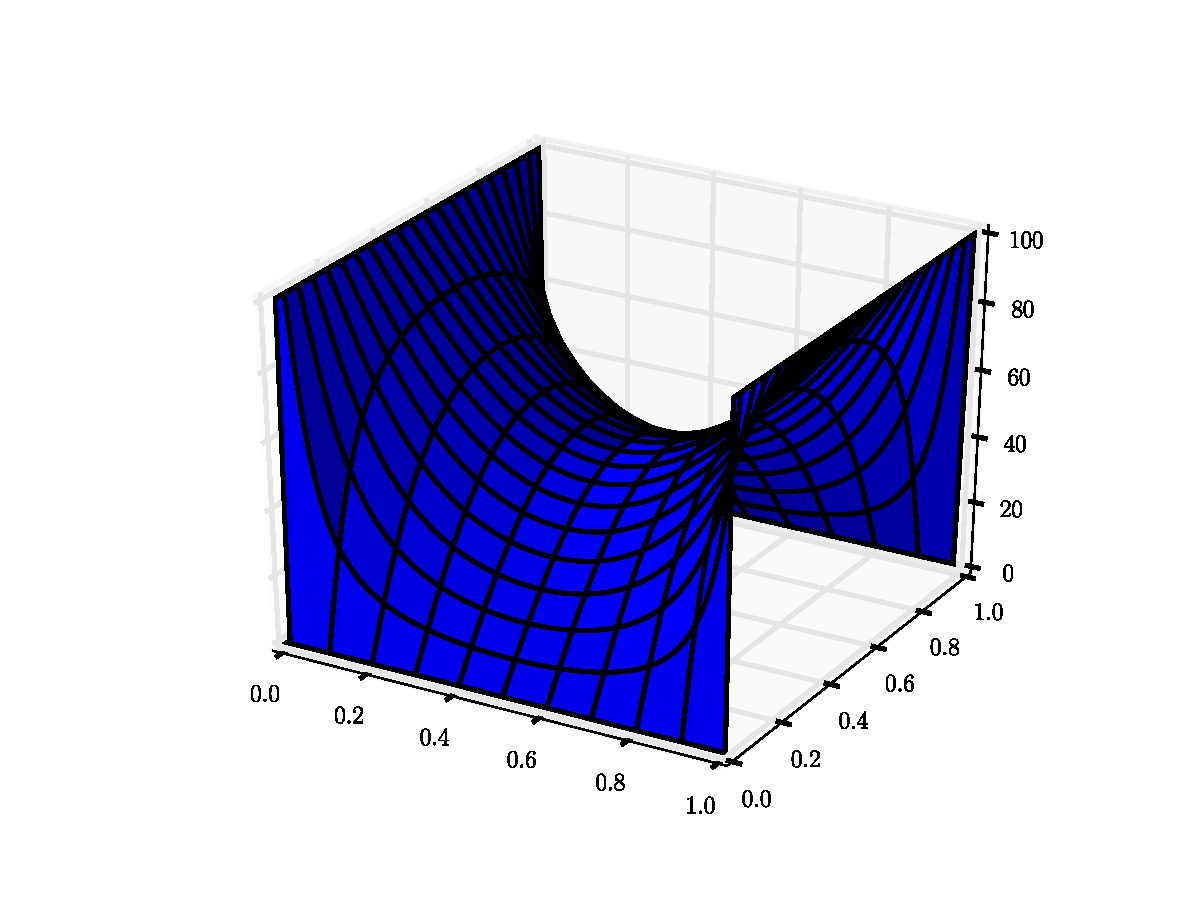
\includegraphics[width=.75\textwidth]{laplace.pdf}
\end{figure} 
\end{problem}


\section*{Conclusion} % =======================================================

% TODO: Revise this section.
Refer often to NumPy's documentation.
If there's something simple you would like to with an array, there's probably already a way to do it built in to NumPy.

The following online resources are specific to SciPy:
\begin{itemize}
\item Official SciPy Documentation (\url{http://docs.scipy.org/doc/})
\item Sections 1.3 and 1.5 of the SciPy Lecture Notes (\url{http://scipy-lectures.github.io/})
\end{itemize}

\newpage

\section*{Additional Material} % ==============================================

\subsection*{Random Sampling} % -----------------------------------------------

The submodule \li{np.random} holds many functions for creating arrays of random values chosen from probability distributions such as the uniform, normal, and multinomial distributions.
It also contains some utility functions for getting non-distributional random samples, such as random integers or random samples from a given array.

% Another table here.

\begin{lstlisting}
# 5 uniformly distributed values in the interval [0, 1).
>>> np.random.random(5)
array([ 0.21845499,  0.73352537,  0.28064456,  0.66878454,  0.44138609])

# A 2x5 matrix (2-D array) of integers in the interval [10, 20).
>>> np.random.randint(10, 20, (2,5))
array([[17, 12, 13, 13, 18],
       [16, 10, 12, 18, 12]])
\end{lstlisting}

Some other commonly-used functions are \li{np.random.randn()}, which samples from the normal distribution, \li{np.random.randint()}, which randomly selects integers from a range, and \li{np.random.random_integers()} which returns an array of random integers in a given range.

A table with np.random functions.

\subsection*{Saving and Loading Arrays} % -------------------------------------

% TODO: revise.
It is often useful to save an array as a file.
NumPy provides several easy methods for saving and loading array data.

\begin{table*}[H]
\begin{tabular}{l|l}
\hline
\li{np.save(file, arr)} & Save an array to a binary file \\
\li{np.savez(file, *arrs)} & Save multiple arrays to a binary file \\
\li{np.savetxt(file, arr)} & Save an array to a text file \\
\hline
\end{tabular}
\end{table*}

\begin{table*}[H]
\begin{tabular}{l|l}
\hline
\li{np.load(file)} & Load and return an array from a binary file \\
\li{np.loadtxt(file)} & Load and return an array from text file \\
\hline
\end{tabular}
\end{table*}

Let's practice saving an array to a file and loading it again.
Note that, when saving an array, NumPy automatically appends the extension \li{.npy} if it is not already present.
\begin{lstlisting}
a = np.arange(30)
np.save('test_arr', a)
new_a = np.load('test_arr.npy')
np.savez('test_multi', a=a, new_a=new_a)
arrs = np.load('test_multi.npz')
\end{lstlisting}
The variable \li{arrs} points to a dictionary object with the keys \li{a} and \li{new_a} which reference the arrays that have been saved.
The \li{.npz} file extension is the file type used to store multiple arrays.

\subsection*{Iterating Through Arrays} % --------------------------------------

% TODO: revise.
Iterating through an array negates most speed advantages of NumPy. 
You should avoid doing this whenever possible.
You can often avoid iterating through arrays by using \emph{array broadcasting} and \emph{universal functions}, discussed in the next section.

It is occasionally valid to iterate through an array. 
The function \li{np.nditer()} will create an object that iterates through an array as quickly as possible.

\begin{comment}
\subsection*{Linear Algebra} % ------------------------------------------------
Both NumPy and SciPy have a linear algebra library, but the SciPy library is larger. The SciPy linear algebra library is typically imported as follows:

\begin{lstlisting}
from scipy import linalg as la
\end{lstlisting}

The linear algebra library contains several functions to construct special 
matrices, located in 
\li{linalg.special_matrices}. There are also functions that will invert matrices, find determinants and norms, solve linear systems and least squares problems, and find special matrix decompositions. You can read more about the linear algebra capabilities of SciPy in the 
documentation for the \li{linalg} module found at
\url{http://docs.scipy.org/doc/scipy/reference/linalg.html}.

Finally, the \li{scipy.linalg} library has a \li{matrix} class that is very 
similar to a 2-D NumPy array. The matrix class can be convenient when doing matrix 
operations. However, in such situations we still recommend using NumPy arrrays, which have many of the same features and are also compatible with all other SciPy operations.

The \li{scipy.linalg} library will be essential for the remainder of the labs in this manual. We will address the details of this package at length in future labs. 
\end{comment}

\begin{comment}
\subsection*{Polynomials} % ---------------------------------------------------

The \li{np.poly1d} object represents a polynomial in NumPy.
The constructor is called with the coefficients of the desired polynomial. 

\begin{lstlisting}
>>> poly_array = np.poly1d([3, 5, 1, 2, 0, 1])
>>> print poly_array
   5     4     3     2
3 x + 5 x + 1 x + 2 x + 1
\end{lstlisting}

The object \li{poly_array} represents the polynomial $3x^5+5x^4+x^3+2x^2+1$.
NumPy provides many functions to operate on \li{poly1d} objects (see \url{http://docs.scipy.org/doc/numpy/reference/routines.polynomials.polynomial.html}).

Here is an example using the \li{poly1d} class. Recall that
\[
e^x = \sum_{n=0}^{\infty} \frac{x^n}{n!}.
\]
The following function evaluates the $n^{th}$ partial sum of this series at the value $a$.

\lstinputlisting[style=fromfile]{exp.py}

The last two lines can be condensed by using the following command.

\begin{lstlisting}
np.polyval(p, a)
\end{lstlisting}

\begin{problem}
\leavevmode
\begin{enumerate}
\item Use NumPy's polynomial objects to approximate the following series.
\[
\arcsin x = \sum_{n=0}^{\infty} \frac{\left(2 n\right) ! x^{2 n + 1}}{\left(2 n + 1\right)\left(n!\right)^2 4^n}
\]
This series converges on $(-1, 1)$. Use your series approximation to approximate $\pi$. Hint: think of the powers of $x$ that
are not included in the series as having zero coefficients.

\item The lambert W function is the inverse of $x e^x$.
Its Taylor series is below (note the index starts at 1).
\[
W(x) = \sum_{n=1}^{\infty} \frac{\left(-n\right)^{n-1} x^n}{n!}
\]
This series has a radius of convergence of $\frac{1}{e}$.
Use the series to approximate a number $x$ such that $x e^x = \frac{1}{4}$.
Verify that your approximation is close.
\end{enumerate}
\end{problem}
\end{comment}

\newpage

\section*{NumPy Visual Guide}

\subsection*{Data Access}

The entries of a 2-D array are the rows of the matrix (as 1-D arrays).
To access a single entry, enter the row index, a comma, and the column index.
Remember that indexing begins with $0$.

\begin{align*}
A[0] = \left(\begin{array}{rrrrr}
\tikzmarkin{row1}\times & \times & \times & \times & \times\tikzmarkend{row1}\\
\times & \times & \times & \times & \times\\
\times & \times & \times & \times & \times\\
\times & \times & \times & \times & \times\\
\end{array}\right)
&&
A[2,1] = \left(\begin{array}{rrrrr}
\times & \times & \times & \times & \times\\
\times & \times & \times & \times & \times\\
\times & \tikzmarkin{entry} \times \tikzmarkend{entry} & \times & \times & \times\\
\times & \times & \times & \times & \times
\end{array}\right)
\end{align*}

\subsection*{Slicing}

A lone colon extracts an entire row or column from a 2-D array.
The syntax \li{[a:b]} can be read as ``the $a^{th}$ entry up to (but not including) the $b^{th}$ entry.''
Similarly, \li{[a:]} means ``the $a^{th}$ entry to the end'' and \li{[:b]} means ``everything up to (but not including) the $b^{th}$ entry.''

\begin{align*}
\text{\li{A[1]}} = \text{\li{A[1,:]}} = \left(\begin{array}{rrrrr}
\times & \times & \times & \times & \times\\
\tikzmarkin{row2}\times & \times & \times & \times & \times\tikzmarkend{row2}\\
\times & \times & \times & \times & \times\\
\times & \times & \times & \times & \times\\
\end{array}\right)
&&
\text{\li{A[:,2]}} = \left(\begin{array}{rrrrr}
\times & \times & \tikzmarkin{col}\times & \times & \times\\
\times & \times & \times & \times & \times\\
\times & \times & \times & \times & \times\\
\times & \times & \times\tikzmarkend{col} & \times & \times
\end{array}\right)
\end{align*}

\begin{align*}
\text{\li{A[1:,:2]}} = \left(\begin{array}{rrrrr}
\times & \times & \times & \times & \times\\
\tikzmarkin{block}\times & \times & \times & \times & \times\\
\times & \times & \times & \times & \times\\
\times & \times\tikzmarkend{block} & \times & \times & \times
\end{array}\right)
&&
\text{\li{A[1:-1,1:-1]}} = \left(\begin{array}{rrrrr}
\times & \times & \times & \times & \times\\
\times & \tikzmarkin{interior} \times & \times & \times & \times\\
\times & \times & \times & \times \tikzmarkend{interior} & \times\\
\times & \times & \times & \times & \times\end{array}\right)
\end{align*}

\subsection*{Stacking}

\li{np.hstack()} stacks sequence of arrays horizontally and \li{np.vstack()} stacks a sequence of arrays vertically.

\begin{align*}
A = \left(\begin{array}{ccc}
\times & \times & \times\\
\times & \times & \times\\
\times & \times & \times
\end{array}\right)
&&
B = \left(\begin{array}{ccc}
* & * & * \\
* & * & * \\
* & * & *
\end{array}\right)
\end{align*}

\begin{align*}
\text{\li{np.hstack((A,B,A))}} =
\left(\begin{array}{ccccccccc}
\times & \times & \times & * & * & * & \times & \times & \times\\
\times & \times & \times & * & * & * & \times & \times & \times\\
\times & \times & \times & * & * & * & \times & \times & \times
\end{array}\right)
\end{align*}

\begin{align*}
\text{\li{np.vstack((A,B,A))}} =
\left(\begin{array}{ccc}
\times & \times & \times\\
\times & \times & \times\\
\times & \times & \times\\
* & * & * \\
* & * & * \\
* & * & * \\
\times & \times & \times\\
\times & \times & \times\\
\times & \times & \times
\end{array}\right)
\end{align*}
Because 1-D arrays are flat, \li{np.hstack()} concatenates 1-D arrays and \li{np.vstack()} stacks them vertically.
To make several 1-D arrays into the columns of a 2-D array, use \li{np.column_stack()}.

\begin{align*}
x = \left(\begin{array}{ccc}\times & \times & \times\end{array}\right)
&&
y = \left(\begin{array}{ccc}* & * & *\end{array}\right)
\end{align*}

\begin{align*}
\text{\li{np.hstack((x,y,x))}} =
\left(\begin{array}{ccccccccc}
\times & \times & \times & * & * & * & \times & \times & \times
\end{array}\right)
\end{align*}

\begin{align*}
\text{\li{np.vstack((x,y,x))}} =
\left(\begin{array}{ccc}
\times & \times & \times\\
* & * & *\\
\times & \times & \times
\end{array}\right)
&&
\text{\li{np.column_stack((x,y,x))}} =
\left(\begin{array}{ccc}
\times & * & \times\\
\times & * & \times\\
\times & * & \times
\end{array}\right)
\end{align*}



\subsection*{Broadcasting}

Really only need two pictures here.


% =============================================================================
% =============================================================================
% MATERIAL TO BE MOVED TO OTHER LABS ==========================================
% =============================================================================
% =============================================================================


\begin{comment} % Matplotlib lab vvvvvvvvvvvvvvvvvvvvvvvvvvvvvvvvvvvvvvvvvvvvvv
\li{np.arange()}, NumPy's version of the built-in \li{range()} function, creates evenly-spaced values within an interval specified with slicing syntax.
Specifically, \li{np.arange(start, stop, step)} returns an array of numbers from \li{start} up to (but not including) \li{stop}, with each entry \li{step} apart.
If they are not specified, \li{start} defaults to $0$ and \li{step} defaults to $1$.

\begin{lstlisting}
# The integers from 0 to 5, exclusive.
>>> np.arange(5)
array([0, 1, 2, 3, 4])

# The complex integers from 3 to 8, exclusive.
>>> np.arange(3, 8, dtype=np.complex)
array([ 3.+0.j,  4.+0.j,  5.+0.j,  6.+0.j,  7.+0.j])

# Every 2nd integer from 10 to 20, exclusive.
>>> np.arange(10, 20, 2)
array([10, 12, 14, 16, 18])
\end{lstlisting}

\li{np.linspace()} also create an array of evenly spaced values in a given interval.
Instead of specifying the step size, we specify the number of desired points in the array.
Unlike \li{np.arange()}, the interval includes the endpoint.
This function is used extensively with plotting and finite difference methods.

\begin{lstlisting}
# 4 evenly spaced values between 0 and 32, inclusive.
>>> np.linspace(0, 32, 4) 
array([  0.        ,  10.66666667,  21.33333333,  32.        ])

# 9 evenly spaced values between -1 and 1, inclusive.
>>> np.linspace(-1, 1, 9)
array([-1.  , -0.75, -0.5 , -0.25,  0.  ,  0.25,  0.5 ,  0.75,  1.  ])
\end{lstlisting}
\end{comment} % Matplotlib lab ^^^^^^^^^^^^^^^^^^^^^^^^^^^^^^^^^^^^^^^^^^^^^^^^

\begin{comment} % Matplotlib lab vvvvvvvvvvvvvvvvvvvvvvvvvvvvvvvvvvvvvvvvvvvvvv
\begin{problem}
Write a function which accepts an integer $n$ as input and does the following:
\begin{enumerate}
\item Creates an $n\times n$ array of \li{floats} randomly chosen from a normal distribution
\item Computes the mean of each row (use a built-in command)
\item Computes the variance of these means (use a built-in command).
\end{enumerate}
As you increase $n$, what happens to the output of 
your function? This illustrates one version of
the Law of Large Numbers, about which you will learn more later on.
\end{problem}
\end{comment} % Matplotlib lab ^^^^^^^^^^^^^^^^^^^^^^^^^^^^^^^^^^^^^^^^^^^^^^^^

\begin{comment} % Complexity lab vvvvvvvvvvvvvvvvvvvvvvvvvvvvvvvvvvvvvvvvvvvvvv
\begin{problem} % Time matrix multiplication.
For a $m\times n$ matrix $A$ with entries $a_{ij}$ and an $n\times l$ matrix $B$ with entries $b_{ij}$, the matrix product $C = AB$ is defined entrywise by the formula:
\[c_{ij} = \sum_{k=1}^N a_{ik}b_{kj}\]

The following function performs matrix multiplication using nested lists without using NumPy.

\begin{lstlisting}
def matrix_multiply(A, B):
    """Calculate the matrix product AB.
    Each parameter is a list of lists.
    """
    # Get the dimensions of the matrices and initialize the new 'matrix'.
    m, n, l = len(A), len(B), len(B[0])
    result = []

    # Calculate each entry of the new matrix.
    for i in range(m):
        for j in range(l):
            result.append(sum([A[i][k] * B[k][j] for k in xrange(n)]))
    return result
\end{lstlisting}

Write a function that times matrix multiplication with the above function, and compare it with numpy.dot().
A random matrix $1000\times 1000$ as a list of lists can be created with
\begin{lstlisting}
a = [[random() for j in xrange(1000)] for i in xrange(1000)]
\end{lstlisting}

\end{problem}


% SIMPLIFIED VERSION OF THE CODE BELOW (don't include from other file)


Iterating through this triple \li{for} loop is very expensive.
NumPy also uses loops, but it uses C loops instead of Python loops.
Compare the difference between the pure Python and the NumPy ways:

% \lstinputlisting[style=fromfile]{arr_mult.py}

Table \ref{table:square_times} documents how long\footnote{You can replicate this experiment yourself. In IPython, you can find the execution time of a line of code by prefacing it with \li{\%timeit}. 
If you aren't using IPython, you will need
to use the timeit function documented here: \url{https://docs.python.org/2/library/timeit.html}.} 
one computer took to square a $k \times k$ matrix in both Python (using the function \li{arr_mult}) and NumPy (using the method you found in Problem \ref{prob:simple1}) for various values of $k$. 
As you can see, NumPy is much faster.
One reason for this is that algorithms in NumPy are usually implemented in C or in Fortran. 

\begin{table}
 \begin{tabular}{|c|l|l|} \hline Data Structure & $k\times k$ & Time (s) \\ \hline 
 Python List    & $10\times10$  & 0.0002758503 \\ 
 \cline{2-3}    & $100\times100$    & 0.1336028576 \\ 
 \cline{2-3}    & $1000\times1000$ & 200.4009799957 \\ 
 %& $1\times1$      & 0.0000181198 \\ 
\hline \hline 
 NumPy Array    & $10\times10$  & 0.0000109673 \\
 \cline{2-3}    & $100\times100$    & 0.0009210110 \\ 
 \cline{2-3}    & $1000\times1000$ & 2.1682999134 \\
 %& $1\times1$      & 0.0000298023 \\ 
 \hline \end{tabular}
 \caption{Time for one computer to square a $k \times k$ matrix in Python and NumPy.}
\label{table:square_times} 
\end{table} 
% 

NumPy is optimized for fast array computations.

\end{comment} % Complexity Lab ^^^^^^^^^^^^^^^^^^^^^^^^^^^^^^^^^^^^^^^^^^^^^^^^
